\section{Introduction} \label{sec:introduction}

Many common tasks in prediction modeling can be viewed as a form of counterfactual prediction. First, prediction models are often deployed in settings that are different from those in which they are trained. One of the ways settings may differ is that treatment policies or patterns after baseline may vary, particularly for models with a longer time horizon for prediction \cite{van_geloven_prediction_2020}. For example, a model fit in a setting where 5\% are treated over the follow up period may not produce valid predictions in a setting where 50\% are treated and vice versa. Even when models are deployed in the same setting, treatment policies may change over time, affecting who is likely to be treated and leading to problems of ``domain adaption'' or ``dataset shift'' \cite{finlayson_clinician_2021,subbaswamy_development_2020}. These differences between the training and deployment setting can cause the performance of models to degrade, particularly when, as is often the case, model predictors are themselves correlated with, or direct determinants of, treatment \cite{pajouheshnia_accounting_2017,}. 

When faced with a change in the treatment policies, ideally, one would re-train the model. However, collecting the necessary data in the new setting may be inordinately expensive or time consuming. Absent sufficient resources or as a stop gap, one might consider using the training data to tailor the model to target the expected outcome that would be observed were treatment to be administered as in the deployment setting \cite{dickerman_predicting_2022}. Alternatively, one might want to estimate how poorly the existing model is likely to perform in the deployment setting, to determine whether additional data collection efforts are worthwhile. In either case, the research questions pertain to counterfactual predictions.

Second, there are instances in which the prediction question itself is counterfactual. For instance, clinicians may use a model to counsel patients about their risk of disease if they were to remain untreated or to compare risks under alternative treatment strategies \cite{lin_scoping_2021,schulam_reliable_2017-1}. In some circumstances, such as when data from a randomized trial are used to model the conditional average treatment effect, this can be done without any additional formalism. However, as often is the case, when training data are obtained in an observational setting where treatment initiation over follow up is not strictly controlled by the investigator, the predictions most relevant to decision-making are counterfactual \cite{dickerman_counterfactual_2020,schulam_reliable_2017-1}. 

In both instances, we need methods for tailoring models to answer counterfactual prediction questions, even when data on the full set of potential outcomes is not available. We also need performance metrics that agnostically evaluate model performance in these new environments without assuming the prediction model is correctly specified.

Here, we examine the conditions under which tailoring a model to counterfactual prediction is possible using training data alone. Under similar conditions, we also show that the counterfactual performance of the model may be estimated independently from the method used to fit the model and may be evaluated even if the model is misspecified. Performance measures may therefore be used to differentiate between better and worse-performing models or to quantify how badly a model is likely to perform in a new setting.


\section{Set up and notation} \label{sec:setup}
Let $Y$ be the outcome of interest, $X$ a vector of baseline covariates, and $A$ an indicator of treatment over the follow up period. We assume that data are obtained from a simple random sample from a target population $\{(X_i, A_i, Y_i)\}_{i=1}^n$ in which initiation of treatment follows some course $f^*(A | X)$. Covariates in $X$ include a set sufficient to control confounding of the treatment-outcome relationship ($L$) as well as additional predictors of the outcome ($P$). Our goal is to build a prediction model for $Y$ using only covariates $X^*$ which are a subset of $X$, i.e. $X^* \subset X$, and chosen based on their availability and prediction potential rather than strictly based on whether they control confounding (Note that $X^*$ can include components of both $L$ and $P$). For now, the treatment $A$ is a point treatment, i.e. treatment is initiated after baseline and sustained throughout or its effect is independent of duration. In the Appendix, we extend our setup to handle time-varying treatments. We also assume that there is no loss to follow up, but our results can be extended by recognizing censoring is like a time-varying treatment. An example directed acyclic graph for this process is shown in Figure \ref{fig:dag1}. 

\begin{figure}[t]
    \centering
    \begin{tikzpicture}[> = stealth, shorten > = 1pt, auto, node distance = 2.5cm, inner sep = 0pt,minimum size = 0.5pt, semithick]
    \tikzstyle{every state}=[
      draw = white,
      fill = white
    ]
    \node[state] (l0) {$L$};
    \node[state] (a0) [right of=l0] {$A$};
    \node[state] (y1) [right of=a0] {$Y$};
    \node[state] (p0) [below of=l0] {$P$};
    \node[state] (u0) [above of=l0] {$U$};

    \path[->] (l0) edge node {} (a0);
    \path[->] (l0) edge [out=20, in=160, looseness=1.5] node {} (y1);

    \path[->] (a0) edge node {} (y1);
    
    \path[->] (p0) edge node {} (y1);

    \path[->] (u0) edge node {} (y1);
    \path[->] (u0) edge node {} (l0);
    \end{tikzpicture}
    \caption{Example directed acyclic graph for prediction in a setting with a single time fixed treatment $A$ over follow up.}
    \label{fig:dag1}
\end{figure}

The data are randomly split into a training set and a test set with $n = n_{train} + n_{test}$. Let $D_{train}$ and $D_{test}$ be indicators of whether an observation is in the training set or test set respectively. As is customary, we use the training set to build a prediction model for the expected outcome conditional on covariates $\E[Y | X^*]$ and, then use the test set to evaluate model performance. Our results, however, apply equally to existing prediction models or biomarkers, in which case splitting is not necessary. Let $\mu_{\beta}(X^*)$ be a parametric model, indexed by parameter $\beta$, and $\mu_{\widehat{\beta}}(X^*)$ be the ``fitted'' model using parameter estimates $\widehat{\beta}$. We allow for the possibility that model $\mu_{\beta}(X^*)$ is \textit{misspecified}. For a particular estimand such as $\E[Y | X^*]$, a model is correctly specified if there exists $\beta_0 \in \mathcal{B}$, where $\mathcal{B}$ is the parameter space of $\beta$, such that $\mu_{\beta_0}(X^*) = \E[Y | X^*]$ and the model is misspecified if no such $\beta_0$ exists.  In several places, we use $f(\cdot)$ generically to denote densities.

To define counterfactual estimands of interest, let $Y^a$ be the potential outcome under an intervention which sets treatment $A$ to $a$. To keep our notation simple, here we limit our focus to point treatments that are \textit{static} and \textit{deterministic}, but extend to \textit{random} and \textit{dynamic} regimes, such as those mentioned in the introduction, in the appendix. 

In the Appendix, we extend these results to the case that treatment is time-varying (section \ref{sec:timevarying}) as well as when the counterfactual intervention is posed as a random or dynamic regime rather than a static regime (section \ref{sec:randomdynamic}). These may be more relevant for some real world prediction tasks, for instance, when evaluating the performance of models for treatment naive risk over a long follow up period in which people start and stop treatment. 

\section{Training and performance estimands} \label{sec:targets}
Our goal is to a model for counterfactual prediction under hypothetical shifts in treatment policy and determine the model's performance. We posit a parametric prediction model $\mu_{\beta}(X^*)$ for the expected potential outcome conditional on covariates $\E[Y^a | X^*]$, which we wish to estimate from the training dataset. The model may be misspecified, such as if, for instance, it is a model trained on another target such as the expected (factual) outcome in the source population $\E[Y | X^*]$.

To determine the performance of the model, a number of common performance measures are available in the prediction literature \cite{harrell_multivariable_1996, altman_what_2000, steyerberg_clinical_2019}. These measures generally compare fitted predictions $\mu_{\widehat{\beta}}(X^*)$ and the true outcomes $Y^a$ via some distance function and associated sample statistic. However, for counterfactual predictions, model evaluation is not as simple because the potential outcome $Y^a$ is not directly observed. Yet, as we will show, under certain conditions the expected value of the performance measure may still be identified from the observed data in the test set. An example performance measure of interest is 
\begin{equation*}
    \psi = \E[(Y^a - \mu_{\widehat{\beta}}(X^*))^2 \mid D_{test} = 1]
\end{equation*}
where the squared error loss $(Y^a - \mu_{\widehat{\beta}}(X^*))^2$ quantifies the discrepancy between the potential outcome under treatment level $A = a$ and the model prediction $\mu_{\widehat{\beta}}(X^*)$ in terms of the squared difference. In the main text, we focus on the mean squared error as the performance measure of interest $\psi$. In the Appendix, we extend our results to the case where $\psi$ is any member of a generic class of counterfactual loss functions $L(Y^a,  \mu_{\widehat{\beta}}(X^*))$ (Section \ref{sec:tf_proof}) as well as more complex risk-based metrics such as area under the receiver operating characteristics curve (AUC, Section \ref{sec:auc}), which depends on paired observations, and the calibration curve (Section \ref{sec:calib}), which is a functional. Importantly, all are identifiable without assuming $\mu_{\widehat{\beta}}(X^*)$ is correctly specified.

\section{Identifiability conditions} \label{sec:identifiability}
We will assume the following identifiability assumptions which have been described in more detail elsewhere \cite{hernan_causal_2020, robins_new_1986, robins_graphical_1987}.

\begin{enumerate}
    \item[A1.] \textit{Consistency.} If $A = a$, then $Y^a = Y$ 
    \item[A2.] \textit{Exchangeability.} $Y^a \perp\!\!\!\perp A \mid X$ 
    \item[A3.] \textit{Positivity.} For all $x$, $\Pr[A = a \mid X = x] > 0$ 
\end{enumerate}

Consistency implies that observed outcomes among those with $A = a$ reflect potential outcomes under corresponding level of treatment. It would be violated if, for instance, there were multiple ``hidden'' versions of the treatment under consideration. The exchangeability condition stipulates that treatment is conditionally independent of the potential outcome given covariates $X$. Finally, the positivity condition implies that there is a positive probability of observed treatment level $A = a$ in all strata of $X$.  

\section{Tailoring a model for counterfactual predictions} \label{sec:model}

As we show in Appendix Section \ref{sec:model_proof}, under the conditions above $\E[Y^a | X^*]$ is identified by
\begin{equation}\label{eqn:estimand1}
    \phi_a(X^*) \equiv \E[\E[Y \mid X, A = a, D_{train} = 1] \mid X^*, D_{train} = 1]
\end{equation}
or, equivalently, using an inverse probability weighted expression 
\begin{equation}\label{eqn:estimand2}
    \phi_a(X^*) = \E\left[\frac{I(A = a)}{\Pr[A = a \mid X, D_{train} = 1]} Y \Big| X^*, D_{train} = 1\right]
\end{equation}
The two expressions for $\phi_a(X^*)$ suggest possible approaches for tailoring the model for counterfactual predictions using only the training data. 

One approach, based on equation \ref{eqn:estimand1} is to subset to participants with corresponding treatment level $A = a$ in the training data and fit a model $\mu_\beta(X)$ for the observed $Y$ conditional $X$, i.e. $\E[Y | X, A = a] = \mu_\beta(X)$. Then when the desired predictors $X^*$ are a subset of $X$, the covariates sufficient to ensure exchangeability,  predictions are marginalized (standardized) over the covariates in $X$ that are not in $X^*$. The resulting predictions will be consistent for $\E[Y^a \mid X^*]$ provided $\mu_\beta(X)$ is correctly specified. An alternative suggested in \cite{dickerman_predicting_2022}, would be to simulate samples from $\mu_\beta(X)$ and fit a second stage model $\mu^*_\beta(X^*)$ using only the subset of the predictors of interest.  

A second approach, based on \ref{eqn:estimand2} is to fit a weighted model $\mu_\beta(X^*)$, using for instance weighted maximum likelihood, with weights equal to the probability of receiving treatment level $A = a$ conditional on covariates $X$ necessary to ensure exchangeability, i.e. $W = \frac{I(A = a)}{\Pr[A = a \mid X, D_{train} = 1]}$. This is the basis for previously proposed methods for counterfactual prediction based on inverse probability of treatment weighting \cite{sperrin_using_2018,van_geloven_prediction_2020}. Note that, as before, it is possible to specify a subset of predictors $X^*$ used in the prediction model $\mu_\beta(X^*)$ as compared to the full set of covariates $X$ required for exchangeability which are only necessary for defining the weights $W$, however a second marginalization or simulation step is not required. This means tailoring the model for counterfactual predictions using the weighting approach can be accomplished more easily using off-the-shelf software.


%%%%%%%%%%%%%%%%%%%%%%%%%%%%%%%%%%%%%%%%%%%%%%%%%%%%%%%%%%%%%%%%%%%%%%%%%%%
\section{Assessing model performance} \label{sec:performance}
%%%%%%%%%%%%%%%%%%%%%%%%%%%%%%%%%%%%%%%%%%%%%%%%%%%%%%%%%%%%%%%%%%%%%%%%%%%

Using the same identifiability conditions, in Appendix Section \ref{sec:tf_proof}, we show the model performance metric $\psi$ is identifiable using data from the test set through the expression
\begin{equation}\label{eqn:mse1}
    \psi(a) \equiv \E\left[\E[(Y - \mu_{\widehat{\beta}}(X^*))^2 \mid X, A=a, D_{test} = 1] \mid D_{test} = 1\right]
\end{equation}
or, equivalently, using an inverse probability weighted expression, 
\begin{equation}\label{eqn:mse2}
    \psi(a) = \E\left[\frac{I(A = a)}{\Pr[A = a \mid X, D_{test} = 1]}(Y - \mu_{\widehat{\beta}}(X^*))^2 \mid D_{test} = 1\right]
\end{equation}
regardless of whether the model $\mu_{\widehat{\beta}}(X^*)$ has been tailored to target $\E[Y^a \mid X]$ or is correctly specified in general. 

As before, the two expression suggest two different approaches for the estimation of model performance using the test data alone. 

First, using the sample analog of expression (\ref{eqn:mse1}), an estimator of the target MSE is 
\begin{equation}\label{eqn:cl_estimator}
    \widehat{\psi}_{CL}(a) = \frac{1}{n_{test}} \sum_{i=1}^nI(D_{test, i} = 1)\widehat{h}_a(X_i)
\end{equation}
where $\widehat{h}_a(X)$ is an estimator for the conditional loss $\E[(Y - \mu_{\widehat{\beta}}(X^*))^2 \mid X, A=a, D_{test} = 1]$ and from the perspective of estimating $\psi(a)$ may be considered a nuisance function. To keep notation simple, we suppress the dependency of $\widehat{h}_a(X)$ on $\mu_{\widehat{\beta}}$. When the dimension of $X$ is small it may be possible to use sample analogs of $\widehat{h}_a(X)$. In almost all practical cases though some form of modeling will be required, in which case, $\widehat{\psi}_{CL}(a)$ is a consistent estimator for $\psi(a)$ as long as $\widehat{h}_a(X)$ is correctly specified.

Next, using the sample analog of expression (\ref{eqn:mse2}), an alternative weight-based estimator of the target MSE is 
\begin{equation}\label{eqn:ipw_estimator}
    \widehat{\psi}_{IPW}(a) = \frac{1}{n_{test}} \sum_{i=1}^n \frac{I(A_i = a, D_{test, i} = 1)}{\widehat{e}_a(X_i)}(Y_i - \mu_{\widehat{\beta}}(X^*_i))^2
\end{equation}
where $\widehat{e}_a(X)$ is another nuisance function estimating the probability of receiving treatment level $A = a$ conditional on $X$, i.e. $\Pr[A = a \mid X, D_{test} = 1]$. Again, when the dimension of $X$ is small it may be possible to use the sample analog of $\widehat{e}_a(X)$, but in all practical cases, it will have to be modeled. The weighting estimator $\widehat{\psi}_{IPW}$ is a consistent estimator of $\psi$ as long as $\widehat{e}_a(X)$ is correctly specified.

The conditional loss estimator (\ref{eqn:cl_estimator}) relies on correctly specifying the model for the conditional loss and the weighting estimator (\ref{eqn:ipw_estimator})  relies on correctly specifying the model for the probability of treatment. In some settings, one estimator may be preferred over the other when more is known about how treatment is initiated or how the outcome arises, such as when the algorithm for administering treatment is clearly defined. In practice, however, both may be difficult to specify correctly. Using data-adaptive and more flexible machine learning estimators for estimation of these nuisance models offers the possibility of capturing arbitrarily complex data generation processes. These data-adaptive estimators generally have slower rates of convergence than the $\sqrt{n}$ rates of parametric models and therefore will not yield asymptotically valid confidence intervals \cite{chernozhukov_doubledebiased_2018}. An alternative is to use a doubly-robust estimator which combines models for the conditional loss $\widehat{h}_a(X)$ and the probability of treatment $\widehat{e}_a(X)$, such as
\begin{equation}
    \widehat{\psi}_{DR}(a) = \frac{1}{n_{test}} \sum_{i=1}^n I(D_{test,i} = 1) \left[ \widehat{h}_a(X_i) + \frac{I(A_i = a)}{\widehat{e}_a(X_i)} \left\{ (Y_i - \mu_{\widehat{\beta}}(X^*_i))^2 - \widehat{h}_a(X_i)\right\}\right]
\end{equation}
As we show in Appendix section \ref{sec:dr}, under mild regularity conditions \cite{robins_higher_2008}, this estimator will be consistent if one of $\widehat{h}_a(X)$ and $\widehat{e}_a(X)$ is correctly specified. It also permits the use of machine learning or data-adaptive estimators that converge at rate slower than $\sqrt{n}$, thus allowing for more flexible estimation of the nuisance functions. This is due to the fact that the empirical process terms governing the convergence of $\widehat{\psi}_{DR}$ involve a product of the estimation errors for $\widehat{h}_a(X)$ and $\widehat{e}_a(X)$ which converge under the weaker condition that only the \textit{combined} rate of convergence for both nuisance functions is at least $\sqrt{n}$ \cite{chernozhukov_doubledebiased_2018}.

%%%%%%%%%%%%%%%%%%%%%%%%%%%%%%%%%%%%%%%%%%%%%%%%%%%%%%%%%%%%%%%%%%%%%%%%%%%
\section{Model and tuning parameter selection} \label{sec:selection}
%%%%%%%%%%%%%%%%%%%%%%%%%%%%%%%%%%%%%%%%%%%%%%%%%%%%%%%%%%%%%%%%%%%%%%%%%%%

Up to this point, we have assumed that $\mu_{\beta}(X^*)$ is a pre-specified parametric model and ignored any form of model selection (e.g. variable or other specification search) or data-adaptive tuning parameter selection, which may be the case when using an existing (validated) model. In many cases, however, analysts have to select between multiple models or perform a data-adaptive search through a parameter space for tuning parameter selection when developing a prediction model \cite{steyerberg_clinical_2019}. To avoid overfitting, analysts typically use methods such as cross-validation or the bootstrap to perform selection. These techniques rely on optimizing some measure of model performance, such as the MSE.

When performing model or tuning parameter selection for counterfactual prediction, the results from the previous sections suggest that the model performance measure should be targeted to the counterfactual performance in a population in which the hypothetical intervention were universally applied. For example, when using cross-validation for model selection the analyst splits the data into $K$ mutually exclusive ``folds'' and estimates the candidate models using $K - 1$ of the folds and estimates the performance of each in the held out fold. This process is repeated $K$ times where each fold is left out once. The final estimate of performance is the average of the $K$ estimates and the model with best overall performance is selected (or, alternatively, the tuning parameter with the best performance). When targeting counterfactual predictions, at each stage in the procedure the analyst should use modified performance measures such as those in section \ref{sec:performance} above. Failure to do so, can lead to sub-optimal selection with respect to the counterfactual prediction of interest. 

%\section{Time-varying treatments} \label{sec:time-varying}

\section{Simulation experiments} \label{sec:simulation}
We performed two Monte Carlo simulation experiments to illustrate (i) the benefits of tailoring models to the correct counterfactual estimand of interest, (ii) the potential for bias when using naive estimators of model performance such as the MSE, (iii) the importance of correct specification of the nuisance models when estimating counterfactual performance, and (iv) the properties of the doubly-robust estimator under misspecification of the nuisance models. We adapt data generation processes previously used for transporting models between settings under covariate shift \cite{steingrimsson_transporting_2023, morrison_robust_2022}.

\subsection{Experiment 1}
We simulated treatment initiation at baseline based on the logistic model $\Pr[A=1 \mid X]=\operatorname{expit} (1.5-0.3 X)$, where predictors $X$ are drawn from $X \sim$ Uniform $(0,10)$. Under this model, about 50\% initiate treatment but those with higher values of $X$ are less likely to start treatment than those with lower values of $X$. We then simulated the outcome using the linear model $Y=1+X+0.5 X^2- 3A + \varepsilon$, where $\varepsilon \sim \mathcal{N}(0, X)$.  We set the total sample size to 1000 and the data were randomly split in a 1:1 ratio into a training and a test set. Note in this model $X$ = $X^*$. The full process may be written:
\begin{align*}
    X & \sim \text{Unif}(0, 10) \\
    A & \sim \text{Bernoulli}\{\operatorname{expit}(-1.5 + 0.3 X)\} \\
    Y & \sim \text{Normal}(1 + X + 0.5 X^2 - 3 A, X)
\end{align*}    
 
Our goal was to estimate a model in the same population where, contrary to fact, treatment was universally withheld, i.e. we targeted $\E[Y^{a=0} \mid X]$. Under this data generating mechanism, the MSE under no treatment is larger than the MSE under the natural course and identifiability conditions 1-3 are satisfied. We considered two specifications of prediction models $\mu_{\beta}(X)$:
\begin{enumerate}
    \item a correctly specified linear regression model that included the main effects of $X$ and $X^2$, i.e. $\mu_{\beta}(X) = \beta_0 + \beta_1 X + \beta_2 X^2$.
    \item a misspecified linear regression model that only included the main effect of $X$, i.e. $\mu_{\beta}(X) = \beta_0 + \beta_1 X$.
\end{enumerate} 
For each specification, we also considered two estimation strategies: one using ordinary least squares regression (OLS) and ignoring treatment initiation and the other using weighted least squares regression (WLS) where the weights were equal to the inverse of the probability of being untreated. As discussed above the latter specifically targets the counterfactual estimand under no treatment. Finally, we considered two approaches for estimating the performance of the models in the test set: a naive estimate of the MSE using observed outcome values, i.e. 
$$\widehat{\psi}_{Naive}(a) = \frac{1}{n_{test}} \sum_{i=1}^n I(D_{test,i} = 1) (Y_i - \mu_{\widehat{\beta}}(X_i))^2,$$ 
and the inverse-probability weighted estimator $\widehat{\psi}_{IPW}(a)$ from section \ref{sec:performance}. For the latter, we fit a correctly specified logistic regression model for $e_a(X)$, i.e. $e_a(X) = \operatorname{expit}(\alpha_0 + \alpha_1 X)$, in the test set to estimate the weights. Lastly, we also calculated the ``true'' MSE under intervention to withold treatment by generating test data under same process as above but forcing $A = 0$ for everyone and then averaging across simulations.

\begin{table}[t]
    \centering
    \caption{Simulation results for experiment 1 comparing the performance of OLS and WLS models using the naive and inverse probability weighting (IPW) estimators of the MSE.}
    \begin{threeparttable}
        \begin{tabular}{p{3cm}R{1.25cm}R{1.25cm}R{1.25cm}}
        \toprule
        Model $\mu_{\beta}(X)$ & Naive & IPW & Truth  \\
        \midrule
        Correct & & & \\
        \hspace{1em}OLS & 2.9 & 3.6 & 3.6\\
        \hspace{1em}WLS & 5.5 & 1.0 & 1.0\\
        \addlinespace[0.25em]
        Misspecified & & & \\
        \hspace{1em}OLS & 16.8 & 17.5 & 17.5\\
        \hspace{1em}WLS & 19.5 & 15.0 & 15.0\\
        \bottomrule
        \end{tabular}
        \begin{tablenotes}
        \item \noindent Correct and misspecified refers to the specification of the  prediction model $\mu_\beta(X)$. OLS = model estimation using ordinary least squares regression (unweighted); WLS = model estimation using weighted least squares regression with weights equal to the inverse probability of being untreated. Results were averaged over 10,000 simulations. The true counterfactual MSE was obtained using numerical methods. 
        \end{tablenotes}
        \end{threeparttable}
    
\end{table}

Table 1 shows the results of the experiment based on 10,000 simulations. In general, correctly specified models yielded smaller average MSE than misspecified models. Comparing the performance of OLS and WLS estimation, when using $\widehat{\psi}_{Naive}(a)$, the naive estimator of the MSE, OLS seemed to produce better predictions than WLS when correctly specified (average MSE of 2.9 vs. 5.5) as well as when misspecified (average MSE of 16.8 vs. 19.5). In contrast, when using $\widehat{\psi}_{IPW}(a)$, the inverse-probability weighted estimate of the MSE, WLS performed better than OLS both when the model was correctly specified (average MSE of 1.0 vs. 3.6) and when misspecified (average MSE of 15.0 vs. 17.5). For reference, in the last column we show the true counterfactual MSE that would be obtained if one had access to the potential outcomes (obtained via numerical methods). We found that the average of the inverse probability weighted estimator across the simulations was equivalent to this quantity for all specifications and for both OLS and WLS estimation. This suggests that only the modified estimators of model performance in section \ref{sec:performance} are able to accurately estimate the counterfactual performance of the model. Indeed, under this data generation process, if one were to use the naive estimator one might erroneously conclude that the OLS model is the better choice.


\subsection{Experiment 2}

In the previous experiment, we assumed the nuisance models for the MSE were correctly specified. We now consider estimation of model performance in the more likely case that nuisance models are misspecified. Using the results from Section \ref{sec:auc} in the Appendix, we also estimate the area under the receiver operating characteristics curve (AUC). We simulated treatment initiation over follow up $A$ based on the logistic model $\operatorname{Pr}[A=1 \mid X]=\operatorname{expit}(0.5 - 2 X_1 + 3 X_1^2 + 2 X_2 - X_3)$, where $X$ is now a vector of predictors drawn from a 3-dimensional multivariate normal with mean vector $\mu = (0.2, 0, 0.5)$ and covariance matrix $\Sigma = \text{diag}(0.2, 0.2, 0.2)$. This resulted in expected treatment initiation over follow up of 55\%. We also simulated a binary outcome from a Bernoulli distribution with mean $\operatorname{expit}(0.2 + 3 X_1 - 2 X_1^2 + 2 X_2 + X_3 - 2 A)$, implying an average probability of the outcome of 66\% among the untreated and 32\% among treated. Again, we set the total sample size to 1000 and randomly split the data in a 1:1 ratio into a training and a test set. 
\begin{align*}
    X & \sim \text{MVN}(\mu, \Sigma) \\
    A & \sim \text{Bernoulli}\left\{\text{expit}\left(0.5 - 2 X_1 + 3 X_1^2 + 2 X_2 - X_3\right)\right\} \\
    Y & \sim \text{Bernoulli}\left\{\text{expit}\left(0.2 + 3 X_1 - 2 X_1^2 + 2 X_2 + X_3 - 2 A\right)\right\}
\end{align*}

Our prediction model was a main effects logistic regression model fit in the training data, i.e. $\mu_\beta\left(X^*\right) = \operatorname{expit}(\beta_0 + \beta_1 X_1 + \beta_2 X_2 + \beta_3 X_3)$. This model was misspecified with respect to the true data generating process. We assessed the counterfactual performance of the model in an untreated population using the AUC and the MSE, which for a binary outcome is equivalent to the Brier score \cite{brier_verification_1950}. In general, positing a parametric model for $h_0(X)=\mathrm{E}[(Y-g\left(X^*\right))^2 \mid X, A=0]$ may be difficult as the outcome is a squared difference. For binary outcomes, however, expanding the square shows that to estimate $h_0(X)$ it is enough to estimate $\operatorname{Pr}[Y=1 \mid X, A=0]$, which is the approach we used. To determine the effect of the specification of nuisance models $e_a(X)$ and $h_a(X)$ on performance estimates, we compared four estimators of AUC and MSE (${\psi}_{Naive}$, ${\psi}_{IPW}$, ${\psi}_{CL}$, and ${\psi}_{DR}$) using different combinations of correctly specified and misspecified models for $e_a(X)$ and $h_a(X)$:
\begin{enumerate}
    \item Correct $e_a(X)$ - main effects logistic regression model with linear and quadratic terms.
    \item Misspecified $e_a(X)$ - main effects logistic regression model with linear terms only terms.
    \item Correct $h_a(X)$ - main effects logistic regression model with linear and quadratic terms.
    \item Misspecified $h_a(X)$ - main effects logistic regression model with linear terms only terms.
\end{enumerate}
Finally, we also considered using more flexible estimation techniques for nuisance terms $e_a(X)$ and $h_a(X)$. Specifically, we fit generalized additive models for both using the \texttt{mgcv} package in $\mathrm{R}$ entering all covariates as splines using the default options in the \texttt{gam} function.

\begin{table}[t]
    \centering
    \footnotesize
    \caption{Simulation results for experiment 2 comparing the performance of the naive, conditional loss (CL), inverse-probability weighting (IPW), and doubly robust (DR) estimators of the MSE and AUC under correct and misspecified nuisance models.}
 
\begin{threeparttable}
    \begin{tabular}{lcccccccc}
    \toprule
    \multicolumn{1}{c}{ } & \multicolumn{4}{c}{MSE} & \multicolumn{4}{c}{AUC} \\
    \cmidrule(l{3pt}r{3pt}){2-5} \cmidrule(l{3pt}r{3pt}){6-9}
    Estimator & Mean & $\sqrt{n}\times\text{SD}$ & $\sqrt{n}\times\text{Bias}$ & Percent & Mean & $\sqrt{n}\times\text{SD}$ & $\sqrt{n}\times\text{Bias}$ & Percent\\
    \midrule
    Naive & 0.207 & 0.176 & -0.140 & -2.1 & 0.742 & 0.491 & -1.335 & -5.4\\
    \addlinespace[0.3em]
    \multicolumn{9}{l}{Correct}\\
    \hspace{1em}CL & 0.212 & 0.333 & 0.015 & 0.2 & 0.783 & 0.767 & -0.045 & \vphantom{1} -0.2\\
    \hspace{1em}IPW & 0.212 & 0.517 & 0.011 & 0.2 & 0.782 & 1.258 & -0.062 & \vphantom{1} -0.3\\
    \hspace{1em}DR & 0.211 & 0.454 & 0.000 & 0.0 & 0.783 & 1.192 & -0.028 & -0.1\\
    \addlinespace[0.3em]
    \multicolumn{9}{l}{$e_a(X)$ misspecified}\\
    \hspace{1em}CL & 0.212 & 0.333 & 0.015 & 0.2 & 0.783 & 0.767 & -0.045 & -0.2\\
    \hspace{1em}IPW & 0.221 & 0.358 & 0.316 & 4.7 & 0.762 & 0.876 & -0.699 & -2.8\\
    \hspace{1em}DR & 0.212 & 0.349 & 0.016 & 0.2 & 0.782 & 0.841 & -0.066 & -0.3\\
    \addlinespace[0.3em]
    \multicolumn{9}{l}{$h_a(X)$ misspecified}\\
    \hspace{1em}CL & 0.217 & 0.356 & 0.194 & 2.9 & 0.777 & 0.803 & -0.224 & -0.9\\
    \hspace{1em}IPW & 0.212 & 0.517 & 0.011 & 0.2 & 0.782 & 1.258 & -0.062 & -0.3\\
    \hspace{1em}DR & 0.211 & 0.625 & 0.001 & 0.0 & 0.783 & 1.317 & -0.024 & -0.1\\
    \addlinespace[0.3em]
    \multicolumn{9}{l}{Both misspecified}\\
    \hspace{1em}CL gam & 0.213 & 0.348 & 0.052 & 0.8 & 0.782 & 0.800 & -0.063 & -0.3\\
    \hspace{1em}IPW gam & 0.214 & 0.422 & 0.075 & 1.1 & 0.778 & 1.032 & -0.181 & -0.7\\
    \hspace{1em}DR gam & 0.211 & 0.403 & 0.010 & 0.1 & 0.784 & 0.966 & -0.021 & -0.1\\
    Truth & 0.211 & &  &  & 0.784 & &  & \\
    \bottomrule
    \end{tabular}
    \begin{tablenotes}
    \item Average of estimates, estimated bias, estimated standard deviation (SD), and estimated relative bias for the naive empirical, weighting (IPW), conditional loss (CL), and doubly robust (DR) estimators. $\sqrt{n}$ is the number of observations in the test set. Here, $h_a(X)$ is a model for $\operatorname{Pr}[Y=1 \mid X, A=a]$ and $e_a(X)$ denotes a model for $\Pr[A = a|X]$. Relative bias is calculated as $(\text{estimator} -\text{truth})/\text{truth}$. Correct and Misspecified refer to the nuisance models, $e_a(X)$ or $h_a(X)$ or both. In the final rows, gam indicates that a generalized additive model was used to estimate nuisance models. Results were averaged over 10,000 simulations.
    \end{tablenotes}
    \end{threeparttable}
\end{table}

Table 2 shows the results from experiment 2. As in the previous experiment, the naive empirical estimators of the AUC and MSE were biased relative to the true counterfactual values with a relative bias of 2.1\% and $-5.4\%$ respectively. When all models were correctly specified, the weighting, conditional loss, and doubly robust estimators were all unbiased (absolute relative bias between 0.2\% to 0.3\%). When $e_a(X)$ was misspecified, the weighting estimator was biased (relative bias of 4.7\% and -2.8\%) but the conditional loss and doubly robust estimator were unbiased (absolute relative bias of 0.2\% to 0.3\%). Under misspecification of $h_a(X)$, the conditional loss estimator was biased (relative bias of 2.9\% and -0.9\%), but the weighting estimator and the doubly robust estimator were unbiased (absolute relative bias of 0.0\% to 0.3\%). When both models $e_a(X)$ and $h_a(X)$ were misspecified all estimators, including the doubly robust estimator, were biased. Finally, when a more flexible generalized additive model was used to estimate both $e_a(X)$ and $h_a(X)$, the doubly robust estimator was unbiased (absolute relative bias of 0.1\%). Across all scenarios, the weighting estimator generally had the largest standard errors and the conditional loss estimator had the smallest standard errors.




%%%%%%%%%%%%%%%%%%%%%%%%%%%%%%%%%%%%%%%%%%%%%%%%%%%%%%%%%%%%%%%%%%%%%%%%%%%
\section{Application to prediction of statin-naive risk} \label{sec:results}
%%%%%%%%%%%%%%%%%%%%%%%%%%%%%%%%%%%%%%%%%%%%%%%%%%%%%%%%%%%%%%%%%%%%%%%%%%%

We apply the proposed methods to evaluate the performance of two counterfactual prediction models targeting the statin-naive risk of cardiovascular disease: that is the risk in the same population if, contrary to fact, statins had been withheld. We compare one model that was explicitly tailored for the counterfactual estimand of interest and a second that was not. 

\subsection{Study design and data}
The Multi-Ethnic Study on Atherosclerosis (MESA) study is a population-based sample of 6,814 men and women aged 45 to 84 drawn from six communities (Baltimore; Chicago; Forsyth County, North Carolina; Los Angeles; New York; and St. Paul, Minnesota) in the United States between 2000 and 2002. The design, sampling procedures, and collection methods of the study have been described previously \cite{bild_multi-ethnic_2002}. Study teams conducted five examination visits between 2000 and 2011 in 18 to 24 month intervals focused on the prevalence, correlates, and progression of subclinical cardiovascular disease. These examinations included assessments of lipid-lowering medication use (primarily statins), as well as assessments of cardiovascular risk factors such as systolic blood pressure, serum cholesterol, cigarette smoking, height, weight, and diabetes. 

In a previous analysis, we used data from the MESA study to emulate a trial comparing continuous statin use versus no statins benchmarked our results against those from published randomized trials. To construct a model of the statin-naive risk, we then emulated a single arm trial in which no one started statins over a 10-year follow up period. To determine trial eligibility, we followed the AHA guidelines \cite{grundy_scott_m_2018_2019} on statin use which stipulate that patients aged 40 to 75 with serum LDL cholesterol levels between 70 mg/dL and 190 mg/dL and no history of cardiovascular disease should initiate statins if their (statin-naive) risk exceeds 7.5\%. Therefore, we considered MESA participants who completed the baseline examination, had no previous history of statin use, no history of cardiovascular disease, and who met the criteria described in the guidelines (excluding the risk threshold) as eligible to participate in the trial. The primary endpoint was time to atherosclerotic cardiovascular disease (ASCVD), defined as nonfatal myocardial infarction, coronary heart disease death, or ischemic stroke. 

Follow up began at the second examination cycle to enable a ``wash out'' period for statin use and to ensure adequate pre-treatment covariates to control confounding (some were taken from the first cycle and others from the second). In the original analysis, we constructed a sequence of nested trials, however here for simplicity we limited our attention to the first trial. We used the questionnaire in examinations three through five to determine statin initiation over the follow up period. Because the exact timing of statin initiation was not known with precision, we estimated it by drawing a random month between the current and previous examinations. 

Of the 6,814 MESA participants who completed the baseline examination, 4,149 met the eligibility criteria for our trial emulation. There were 288 ASCVD events and 190 non-ASCVD deaths. For the sake of clarity, here we dropped those lost to follow up and ignored competing risks although in practice both can be accommodated in our framework for evaluating the performance of a counterfactual prediction model. For model training and evaluation, we further randomly split the dataset into training and test sets of equal size. 

\subsection{Model estimation and performance}

We compared two prediction models: one that was explicitly tailored to the statin-naive risk and a second that was not. Both models used the same regression specification with main effects of baseline predictors commonly used in cardiovascular risk prediction: age, sex, smoking status, diabetes history, systolic blood pressure, anti-hypertensive medication use and total and HDL serum cholesterol levels.

We tailored the first model for the statin-naive risk using inverse probability of censoring weights. In the emulated single arm trial, statin initiation can be viewed as ``non-adherence'' which can be adjusted for by inverse probability weighting, therefore we censored participants when they initiated statins. To calculate the stablized weights, we estimated two logistic regression models: one for the probability of remaining untreated given past covariate history (denominator model) and one for probability of remaining untreated given the selected baseline predictors (numerator model). The list of covariates in the weight models are given in section \ref{sec:covs} of the Appendix. To create a prediction model for the statin-naive risk, we used the estimated weights to fit a weighted logistic regression model conditional on the baseline predictors of interest. 

For comparison, we fit a second traditional (factual) prediction model by regressing the observed ASCVD event indicator on the same set of baseline predictors, but ignoring treatment initiation over the follow up period. This approach targets the ``natural course'' risk (i.e., the risk under the statin initiation policies that prevailed at the time of the study) rather than the statin-naive risk. We fit the model using standard logistic regression based on maximum likelihood.

To assess the performance of the models, we estimated the naive and counterfactual MSE in the test set. For the latter we used the conditional loss, inverse probability weighting, and doubly robust estimators of the MSE. Models for the initiation of treatment $e_a(X)$ and for the conditional loss $h_a(X)$ were implemented as main effects logistic regression models. As in the simulation example, to estimate the conditional loss it is sufficient to model the probability of the outcome alone. To quantify uncertainty, we used the non-parametric bootstrap with 1000 bootstrap replicates.


\begin{table}[t]
    \centering
    \caption{Estimated MSE in a statin-naive population for two prediction models using emulated trial data from MESA.}
    \begin{threeparttable}
        \begin{tabular}{lcccc}
        \toprule
        \multicolumn{1}{c}{ } & \multicolumn{2}{c}{MSE} & \multicolumn{2}{c}{AUC} \\
        \cmidrule(l{3pt}r{3pt}){2-3} \cmidrule(l{3pt}r{3pt}){4-5}
        Estimator & Logit & Weighted Logit & Logit & Weighted Logit\\
        \midrule
        Naive & 0.069 & 0.072 & 0.710 & 0.708\\
         & (0.003) & (0.003) & (0.013) & (0.014)\\
        CL & 0.086 & 0.085 & 0.719 & 0.727\\
         & (0.005) & (0.004) & (0.015) & (0.015)\\
        IPW & 0.109 & 0.099 & 0.753 & 0.778\\
         & (0.013) & (0.009) & (0.025) & (0.029)\\
        DR & 0.090 & 0.087 & 0.740 & 0.751\\
         & (0.006) & (0.005) & (0.023) & (0.023)\\
        \bottomrule
        \end{tabular}
        \centering
        \begin{tablenotes}[flushleft]
        \item The columns refer to the posited prediction model: Logit is an (unweighted) logistic regression model and weighted logit is a logistic regression model with inverse probability weights for remaining statin-free. The rows are the model performance estimates of the MSE and AUC. Naive is the empirical estimator using factual outcomes ($\widehat{\psi}_{Naive}$), CL is the conditional loss estimator ($\widehat{\psi}_{CL}$), IPW is the inverse probability weighting estimator ($\widehat{\psi}_{IPW}$), DR is the doubly-robust estimator ($\widehat{\psi}_{DR}$). Standard error estimates are shown in parentheses obtained via 1000 bootstrap replicates.
        \end{tablenotes}
        \end{threeparttable}
\end{table}

\subsection{Results}

Table 3 shows estimates of the AUC and MSE and the associated standard errors in a hypothetical statin-naive population for both prediction models using the naive empirical, conditional loss, weighting, and doubly robust estimators. Across both metrics, the conditional loss, weighting, and doubly robust estimators yielded estimates that were greater (30-50\% for MSE, 3-10\% for AUC) than those of the naive empirical estimator, suggesting performance of both models in statin-naive population is worse than in the source population. Of the three estimators of the statin-naive performance, the weighting estimator had greater standard errors than the doubly robust estimator (by 10-100\%) as well as the conditional loss estimator (by 60-160\%). Consistent with the first simulation experiment, the inverse probability weighted logistic model, which was tailored to target the statin-naive risk, performed worse in the source population, but had lower MSE and higher AUC values in the counterfactual statin-naive population. Finally, drawing on the results in section \ref{sec:calib} in the appendix, we estimate the counterfactual calibration of both prediction models in a statin-naive population using a weighted loess estimator where the weights are based on inverse probability of remaining statin free. Figure \ref{fig:calib} shows the results. As expected, the weighted prediction model, which was tailored to target the statin-naive risk, was better calibrated than the unweighted model, which generally underestimated the counterfactual risk.

\begin{figure}[p]
    \centering
    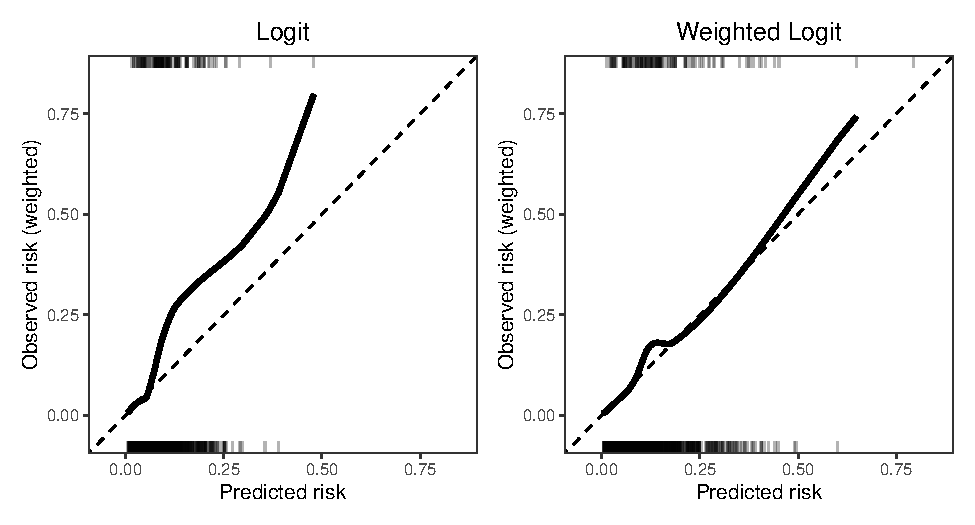
\includegraphics{../3_figures/calib.pdf}
    \caption{Risk calibration curves for counterfactual prediction models fit using logistic regression with and with out inverse probability weights for statin initiation. The rug plot shows distribution of risk predictions among those who develop ASCVD (top) and those who don't (bottom). The black curve is a local-regression smoothed and inverse probability weighted estimate of the calibration curve targeting the statin-naive risk.\label{fig:calib}}
\end{figure}




%%%%%%%%%%%%%%%%%%%%%%%%%%%%%%%%%%%%%%%%%%%%%%%%%%%%%%%%%%%%%%%%%%%%%%%%%%%
\section{Discussion} \label{sec:discussion}
%%%%%%%%%%%%%%%%%%%%%%%%%%%%%%%%%%%%%%%%%%%%%%%%%%%%%%%%%%%%%%%%%%%%%%%%%%%

Many practical problems in prediction modeling may be posed as counterfactual prediction problems, such as when treatment varies between training and deployment or when predictions are meant to inform treatment initiation. Here, we considered cases where counterfactual predictions were desired but only training data from observational sources were available. We described how to tailor models to target counterfactual estimands and the conditions necessary to identify these estimands. Separately, we also discussed how to adjust common measures of model performance to estimate the counterfactual performance of the model under the same hypothetical interventions. Importantly, results for performance measures were valid even when the prediction model is misspecified. A key insight was that for counterfactual prediction standard performance measures will be biased, but performance could be assessed independently from the method used to tailor the model. For loss-based measures of performance, we proposed three estimators for time-fixed treatments based on modeling the conditional loss, the probability of treatment, and a doubly robust estimator that can be used with data-adaptive estimators of either nuisance function. 

In this paper, we have focused on measures of performance under a particular treatment policy. However, prediction models may instead target the estimation of conditional or individualized treatment \textit{effects}, i.e. a comparison between treatment regimes such as $\tau(X^*) = \E[Y^1 - Y^0 \mid X^*]$. In some cases, effects may be easier to communicate to end users or may be desirable to evaluate benefits versus harms of treatment initiation \cite{kent_predictive_2020}. However, absolute means and risks are common outputs of existing prediction models. Several authors have proposed model performance measures for conditional average treatment effects which are identified under similar assumptions to our own \cite{schuler_comparison_2018,rolling2014model,xu_calibration_2022,van2003unified,alaa_validating_2019}. From an estimation standpoint, methods for targeting the conditional average treatment effect and their performance differ from our own because they typically balance estimation of the conditional risk function for the outcome under different treatment levels with the estimation of the treatment effect function, with optimality depending on the relative smoothness of these functionals.

Throughout, we did not assume that the covariates needed to satisfy the exchangeability assumption were the same covariates used in the prediction model. This is important because, in practice,  predictors are often chosen subject to clinical constraints in the data available to end users rather than what would be optimal from a causal (or even predictive) perspective \cite{steyerberg_clinical_2019}. Moreover, methods should reflect the fact that confounding is a problem that needs to be adjusted for in the setting where the model is developed, whereas predictions often need to be optimized for the setting where the model will be applied. 

However, a limitation is that, for we did assume that a sufficient set of covariates could be identified at the time of training to ensure exchanageability. Violations of this assumption are the scope of this study, but it is possible that counterfactual performance metrics could also be identified under alternative conditions. It is also possible to develop sensitivity analyses for exploring how violations of this assumption might affect model performance estimates \cite{robins_sensitivity_2000}.

In this work, we have implicitly assumed that the distribution of predictors is the same in the training and deployment setting. However, in many cases the covariate distributions are likely to differ \cite{bickel_discriminative_2009,sugiyama_covariate_2007}. Like differences in treatment initiation, this may cause the performance of the prediction model to degrade, particularly when the model is misspecified. Methods for transporting prediction models from source to target populations which mirror our own have previously been proposed \cite{steingrimsson_extending_2022, steingrimsson_transporting_2023, li_estimating_2022, morrison_robust_2022}. In future work, it's possible that our results could be integrated with those to allow for both sources of difference between training and deployment.

